% $Id: hardware.tex,v 1.13 2008/05/26 20:01:03 gbauer Exp $

\section{\label{sec:stohard}Storage Manager Design and Hardware}  %Editor: Gerry

\subsection{Overview of Baseline System} 
An overview of the existing  Storage Manager (SM) hardware configuration 
is given in Figure~\ref{fig:system}, and photographs in Fig.~\ref{fig:SMpics}. 
The HLT nodes are grouped in subfarms and connected to two (soon eight) 
gigabit ethernet switches (Force10). 
Data from the HLT is sent to 8 SM logger nodes. 
%The input bandwidth is provided by 6 GigE links per Logger node providing. 
%Currently only 2 switches are connected with 2 GigE links to each Logger node.
% resulting in a total bandwitdh of 2GB/s. 
The Logger nodes are also connected to a GigE switch to provide connectivity 
to the Tier-0 system at CERN.
The connection to the NexSan SATABeasts is provided through two Fibre Channel QLogic SanBox 5600 
switches. Each NexSan SATABeast unit has two controllers with two fiber connections each. 
If one controller fails, traffic is automatically switch to the second controller. 
The total network connectivity from the Logger nodes to the storage units is 8 times 2~Gb, 
such that the system is limited by the performance of the SATABeast controller. 
According to specifications each NexSan SATABeast should be able to reach up to $\sim$400 MB/s write 
or $\sim$800 MB/s read speeds, if equipped with a sufficient number of disks.
A system of 3 SATABeasts should be sufficient to meet a goal of 1 GB/s throughput,
and 6  SATABeasts the storage capacity goal.
However, the 8-fold symmetry of subfarms imposed by the connectivity 
of the 8 Force10 switches implies that efficient utilization of the subfarm resources
suggests a multiple of 4 SATABeasts for balancing the load across the 8 subfarms.

% system overview
\begin{figure}[tb]
\begin{center}  
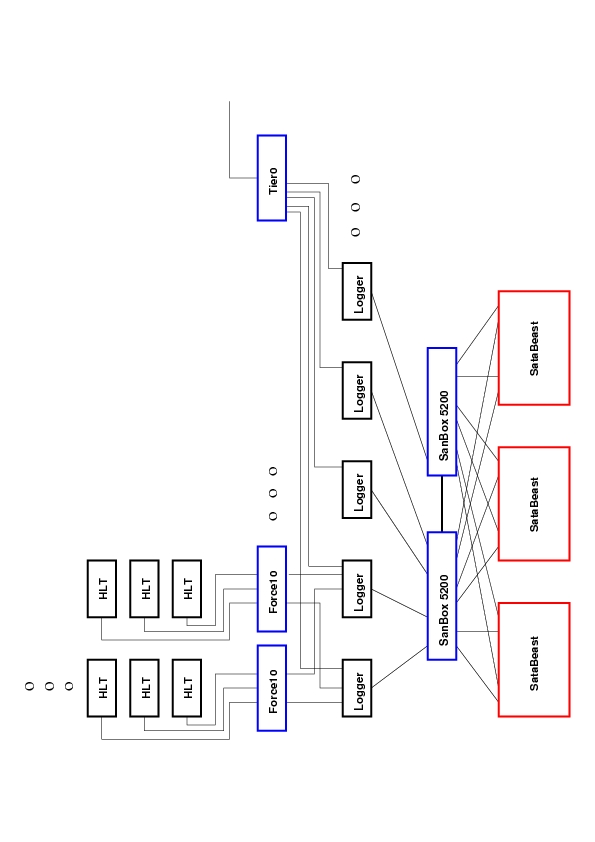
\includegraphics[width=1.0\textwidth]{Hardware/SMsystem}
\caption{\emph{ Storage Manager system overview of the currently installed hardware. 
The leftmost SATABeast is drawn indicating having the arrangement of four disk arrays, 
two arrays of which are ``owned'' by logger node 1 (``L1'') and two by logger node 2 (``L2'').}}
\label{fig:system}
\end{center}
\end{figure}  


% system overview
\begin{figure}[tb]
\begin{center}  
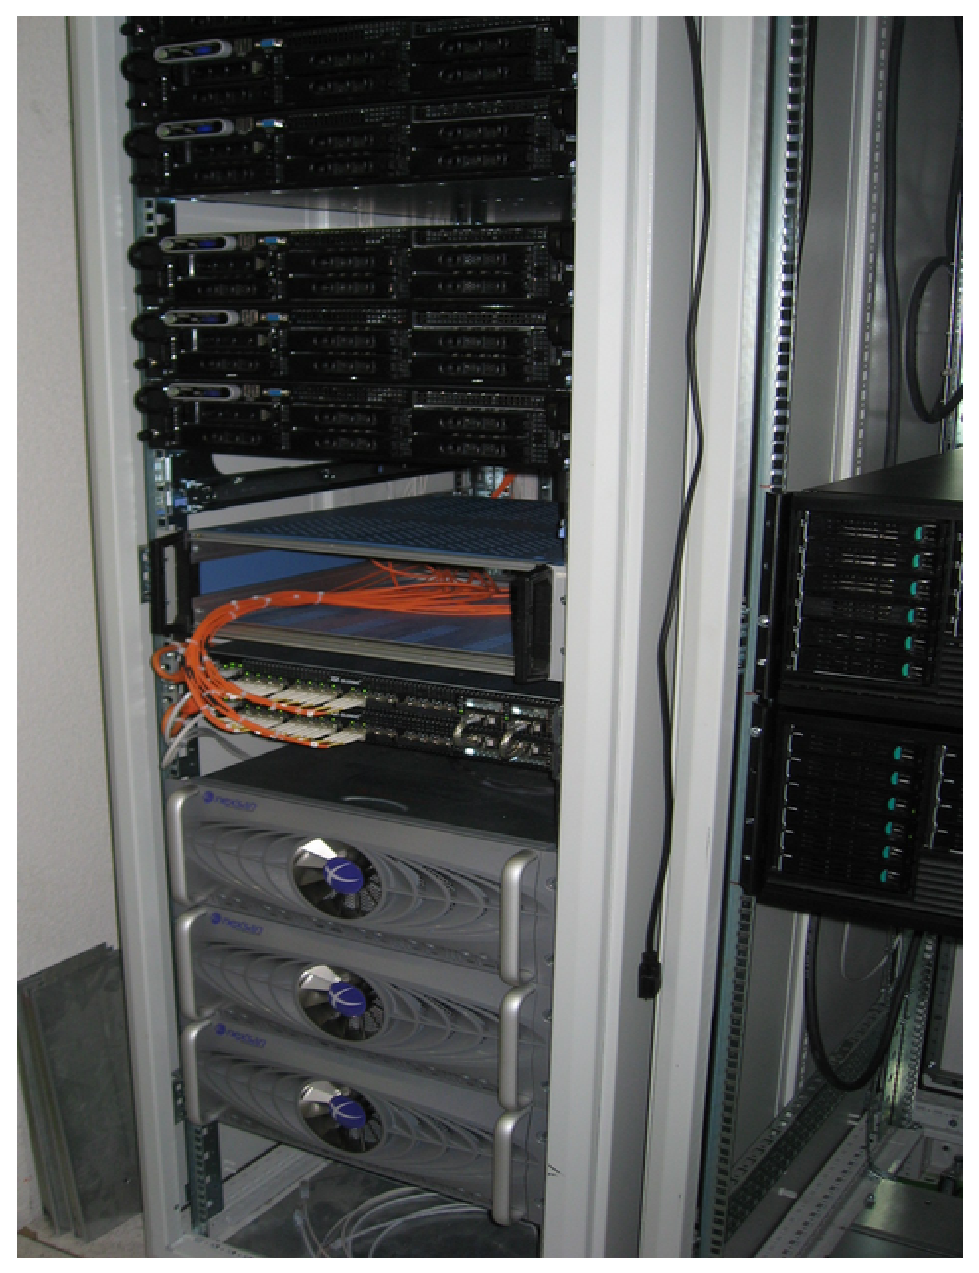
\includegraphics[width=0.48\textwidth]{Hardware/frontSM_img_1385}
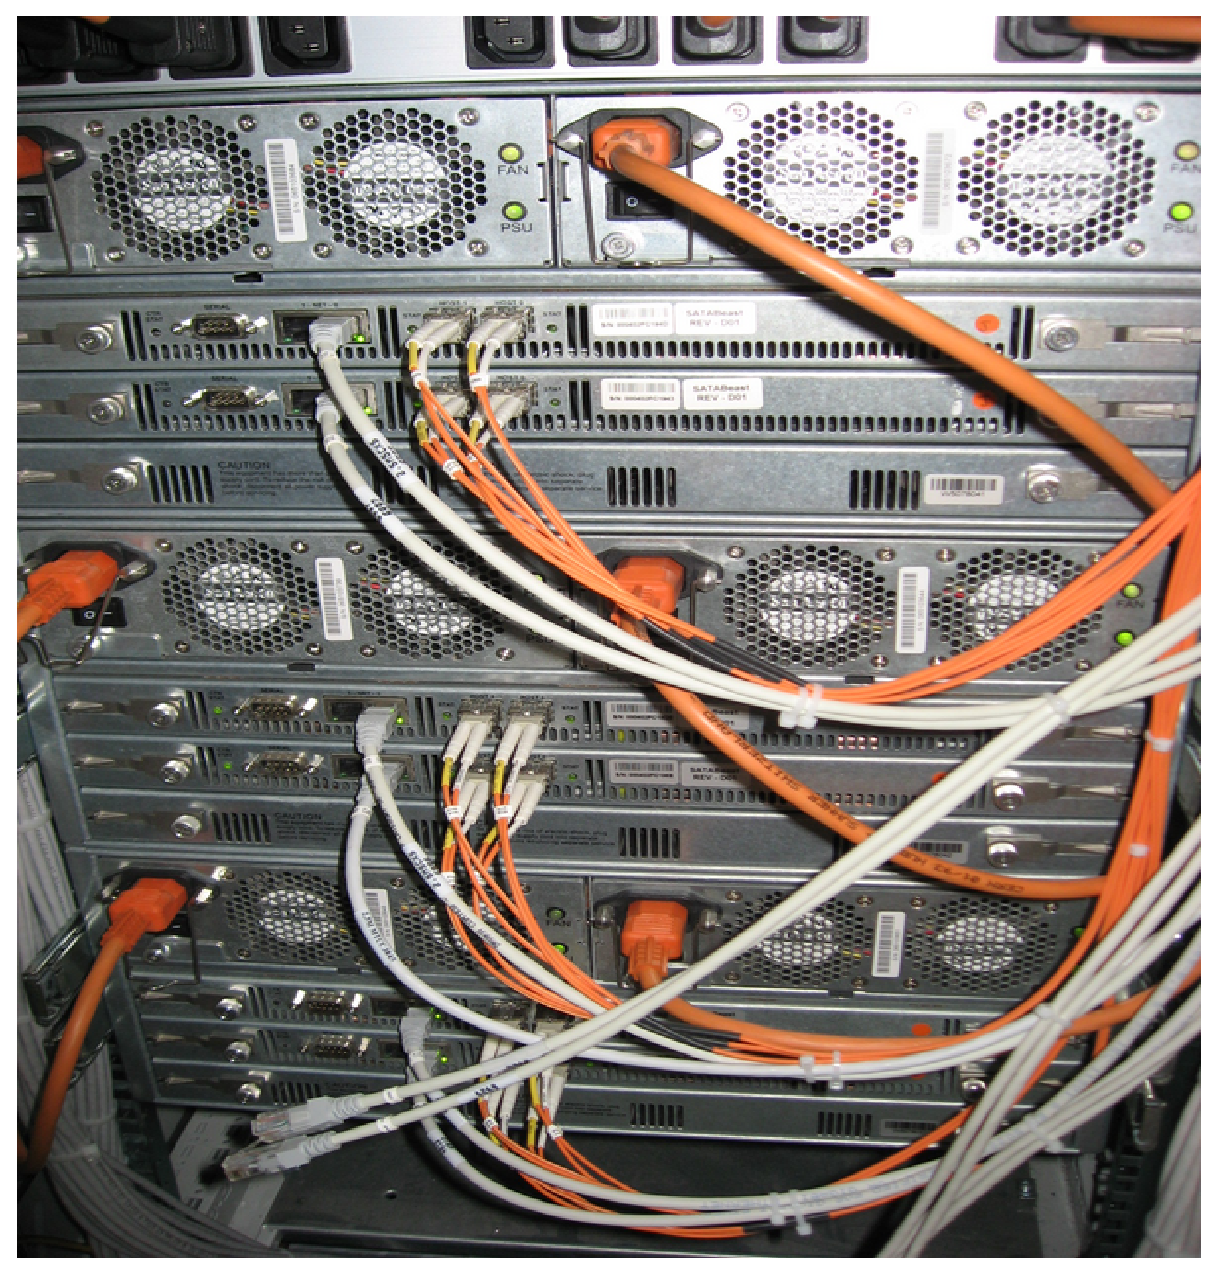
\includegraphics[width=0.48\textwidth]{Hardware/backSMsatacontroller_img_1389}
\caption{\emph{ The Storage Manager system installed at Cessy.
{\bf Left:} View of the front of the SM rack. At the top are the 8 logger nodes 
(only 5 are visible). 
Below the logger nodes  is an empty rectangular box used to help protect 
the bundles of fiber channel cables that are routed inside it to the rear of the rack.
These are connected on the front side of the rack to two Qlogic switches just below. 
The two rows of white fiber connectors  plugged into the switch 
particularly stand-out in the image.
Finally, below the switches are the 3 SATABeast housings.
To the right of this rack is the rack that is foreseen for the new hardware of the expanded system.
{\bf Right:} View of the rear of the 3 SATABeasts. Here one  can see the thick power cords
connected at a given height to a left and right power supply---these are the redundant dual power supply
modules of one SATABeast.
Below the power supplies are two thin modules, one above the other, which are the two controllers.
Each controller is seen to have two fiber cables, these being the 2$\times$ 2 Gb/s links.
To the left of the fiber connections is a single Ethernet connection used for system services.
}}
\label{fig:SMpics}
\end{center}
\end{figure}   




\subsection{Baseline Hardware Components}

\subsubsection{Logger Nodes}
Logger nodes are standard Dell PC's PowerEdge 2950 with two dual-core Xeon processors and 4 GB RAM. 
Each node is equipped with a 4-port GbE card (Silicom PEG4i) and 
a fiber channel host bus adapter (QLogic QLE2460-CK). 
% An additional PCI-e slot is available for an extra 4-port GbE card if needed. 
The same PC's are used for the CMS HLT farm.
The SM nodes are fully incorporated in the DAQ group's Quattor system for managing 
the software installation of PCs, as well as the Nagios system
for monitoring all the DAQ PCs in the \verb+cms+ network.

\subsubsection{Fiber Channel switch}

The fiber channel switches are used to connect the logger nodes and the storage. 
Two QLogic SanBox 5600 switches are used. 
Each chassis includes sixteen 4 Gb ports, plus a four-pack of high-speed 10 Gb ISL ports 
of which one is used to connect the two switches.
The latter interconnect is foreseen to re-route traffic through the other switch
to reconfigure around the hardware failure of certain components.

\subsubsection{Storage Array}

The storage arrays are the SATABeast from NEXSAN. 
Each SATABeast has two controllers with two 2~Gb ports.
The total number of disk slots available is 42 and the system supports Sata disks 
of up to 1~TB size. 
NexSan SATABeasts have been successfully deployed for the CDF Consumer Server Logger system 
at Fermilab since 2006.

The arrangement and allocation of disks in the SATABeast is constrained by a number
of practical considerations.
Without substantial investment in a file management system it is simplest
to dedicate disk arrays to particular logger nodes, and given our use case, 
there is not much incentive to overcome this choice.
Due to its dual controllers, the SATABeast is best fed by two logger nodes,
implying a division of the SATABeast into an even number of disk arrays.
Given the  SATABeast capacity is for 42 disks, and the need for hot spares, 
the obvious choice is a configuration of four 10-disk arrays plus 2 hot spares.
By giving each logger node write control of two arrays, one can also obtain some benefit
from reading and writing from separate arrays, even though we do not plan
to enforce non-overlapping I/O. We can implement such a scheme if it is warranted.
The 10-disk arrays are also appropriate in that much smaller arrays would
suffer reduced throughput, and dramatically larger arrays would be at greater
risk for multi-disk failures, and longer re-build times.
The size of the disk arrays is an issue for some file systems, 
but partitioning the arrays with multiple volumes easily avoids such limitations.
 
\subsubsection{Proxy Server Node}

As discussed extensively in the software section, the SM supplies monitoring
data via a Proxy Server system.
Supplying and maintaining the hardware for the Proxy Server node 
is {\it not} part of the SM project, but a responsibility assumed by the DAQ group.


\subsubsection{Data ``Lookarea''}

It is valuable for commissioning and data monitoring purposes to have rapid
{\it local} access to some fraction of the data recorded.
This has been addressed by copying the very first file of each run 
to a ``Lookarea'' which is locally accessible by users at Cessy.
In the old prototype SM system of  \verb+cmsdisk1+ this was accomplished
by making a Lookarea directory on one of this machines data disks and
exporting to other nodes within the \verb+cms+ network.


For the SATABEast SM, however, we insist upon the policy that users
cannot have {\it any} externally driven interaction with the SM system
in order to protect and preserve the reliability of this real-time critical system.
Thus for the new SM a data disk is exported {\it to} the SM logger nodes
from a non-SM PC, and
the logger node initiates the copy of this first data file to this
external Lookarea machine, i.e. all interaction with the SM is under
SM control.
If the external node is unavailable, the file will not be copied, but
the SM will continue with its normal operation.

The PC serving the Lookarea disk is also a responsibility of the DAQ group.


\subsection{Hardware Expansion\label{sec:SMexpansion}}

The initial Phase-I system assembled in late 2007 was envisaged as Phase-I 
of a three phase expansion, the later phases were primarily to increase the
storage capacity.
Phase-II was to increase the disk inventory by 96 disks to fill up the existing
SATABeasts in the spring of 2008.
Phase-III was foreseen for 2009 to essentially double the system for higher 
luminosity LHC running.
We have been operating under the general philosophy of this plan, 
but two developments have modified its execution.

First, we found that our testing of the system and providing support for CMS
running with a portion of the new SM hardware was significantly hampered 
by the small inventory of disks on hand.
In particular, high data rates to the SATABeast is conditional upon having
fairly large disk arrays.
Therefore the Phase-II disk purchase was accelerated by a few months,
giving us in early April the 118.5 TB currently installed.

Second, CMS management in consultation with DAQ and trigger
project managers concluded that the doubling the system in 2009 would be
better done  for the 2008 LHC run.
Essentially, in this early phase where operation may be unstable 
for the accelerator (e.g. store frequency)
and detector (e.g. triggering, zero-suppression,\ldots), 
it may be very important for CMS to be able to maximize  recording very high data rates
for the limited store-hours available.
The SM hardware team  was thus asked in May to quickly pursue doubling the system.
We have begun the process for purchasing the requested doubling, 
but have also incorporated two secondary design changes.

First, by virtue of the connectivity of the eight FORCE10 switches, the DAQ system
will have an explicit eight-fold symmetry in the data flow.
By having 8 logger nodes, the front end of the SM system is properly matched,
however, 8 nodes feeding 3 SATABeasts is not---the 8 nodes were originally 
conceived as 6 loggers $+$ 2 spares.
The SATABeasts are able to support eight slices,
but doing so breaks the natural topology of one node per  SATABeast controller.
This has the important impact that having 8 rather than 6 nodes will unbalance 
the throughput that the filter farms 
can support, and  the large investment in filter computing resources would be underutilized.
Thus the decision that the  SATABeasts should properly match the 8-fold symmetry
of the greater DAQ system, and that the baseline  configuration should consist
of four  SATABeasts rather than three.

A second modification of the design concerns the robustness of the system.
The Fiber Channel switches that move data from the logger nodes to the 
SATABeasts are fault tolerant, and allow traffic to be routed from one
switch to its partner and still make it to all SATABeasts. 
However, we have already experienced a failure of a switch {\it power supply}
and lost the connections for four of the logger nodes to the  SATABeasts.
To improve fault tolerance the expanded system will equip the logger nodes
with two Fiber Channel connections, one to each switch, so that complete failure of a switch
will not interrupt operation.

Aside from these two alterations, the system expansion is then a simple doubling,
and the final system for 2008 data taking should consist of:
\begin{itemize}
\item 16 logger nodes $+$ 2 hot spares
\item 4 Fiber Channel switches $+$ 1 pre-configured spare
\item 8 SATABeasts fully loaded with 42 disks
\end{itemize}
This system should readily exceed the original throughput/storage goals.

Assuming the purchase process and equipment delivery proceeds in a timely
fashion  the full system should be operational by the fall.


